\documentclass[a4paper,11pt]{jsarticle}


% 数式
\usepackage{amsmath,amsfonts, amssymb}
\usepackage{bm}
% 画像
\usepackage[dvipdfmx]{graphicx}


\begin{document}

\title{巡回符号の課題}
\author{}
\date{\today}
\maketitle


\section{$n=5$の巡回符号}
生成多項式$g(x)$は$1+x^n$の因数なので、
\[
  1+x^5=(1+x)(1+x+x^2+x^3+x^4)
\]
より、$g(x)$の候補は$1+x$と$1+x+x^2+x^3+x^4$
である。
$g(x)=1+x$のときの全ての符号を表\ref{table:n5g1}
に示す。
\begin{table}[hbtp]
  \caption{$g(x)=1+x$の符号}
  \label{table:n5g1}
  \centering
  \begin{tabular}{ccccc}
    00000 &&&& \\
    00011 & 00110 & 01100 & 11000 & 10001 \\
    00101 & 01010 & 10100 & 01001 & 10010 \\
    01111 & 11110 & 11101 & 11011 & 10111
  \end{tabular}
\end{table}
表\ref{table:n5g1}より、$g(x)=1+x$のときの最小ハミング距離は2である。
$g(x)=1+x+x^2+x^3+x^4$のとき、符号は00000と11111のみなので、
最小ハミング距離は5である。

\section{$n=6$の巡回符号}
生成多項式$g(x)$は$1+x^n$の因数なので、
\[
  1+x^6=(1+x^3)^2=(1+x)^2(1+x+x^2)^2
\]
より、$g(x)$の候補を$k$の昇順に並べると
表\ref{table:n6g}になる。
\begin{table}[hbtp]
  \caption{$n=6$の巡回符号の生成多項式}
  \label{table:n6g}
  \centering
  \begin{tabular}{c|l}
    $k$ & $g(x)$ \\ \hline
    1 & $(1+x)(1+x+x^2)^2$ \\
    2 & $(1+x+x^2)^2$ \\
    2 & $(1+x)^2(1+x+x^2)$ \\
    3 & $(1+x)(1+x+x^2)$ \\
    4 & $1+x+x^2$ \\
    4 & $(1+x)^2$ \\
    5 & $1+x$
  \end{tabular}
\end{table}

\section{(8, 4)組織符号}
\begin{eqnarray*}
  p_0 &= u_1 + u_2 + u_3 \\
  p_1 &= u_0 + u_1 + u_2 \\
  p_2 &= u_0 + u_1 + u_3 \\
  p_3 &= u_0 + u_2 + u_3
\end{eqnarray*}
\subsection{生成行列}
\begin{equation*}
  {\bm G}=
  \begin{bmatrix}
    1 & 0 & 0 & 0 & 0 & 1 & 1 & 1 \\
    0 & 1 & 0 & 0 & 1 & 1 & 1 & 0 \\
    0 & 0 & 1 & 0 & 1 & 1 & 0 & 1 \\
    0 & 0 & 0 & 1 & 1 & 0 & 1 & 1
  \end{bmatrix}
\end{equation*}

\subsection{パリティ検査行列}
\begin{equation}
  \label{eq:parity-check-matrix}
  {\bm H}=
  \begin{bmatrix}
    0 & 1 & 1 & 1 & 1 & 0 & 0 & 0 \\
    1 & 1 & 1 & 0 & 0 & 1 & 0 & 0 \\
    1 & 1 & 0 & 1 & 0 & 0 & 1 & 0 \\
    1 & 0 & 1 & 1 & 0 & 0 & 0 & 1
  \end{bmatrix}
\end{equation}

\subsection{最小ハミング距離}

\begin{table}[hbtp]
  \caption{情報源と符号の対応}
  \label{table:all-code}
  \centering
  \begin{tabular}{|cc|}
    \hline
    情報源 & 符号 \\ \hline \hline
    0000 & 00000000 \\ \hline
    0001 & 00011011 \\ \hline
    0010 & 00101101 \\ \hline
    0011 & 00110110 \\ \hline
    0100 & 01001110 \\ \hline
    0101 & 01010101 \\ \hline
    0110 & 01100011 \\ \hline
    0111 & 01111000 \\ \hline
    1000 & 10000111 \\ \hline
    1001 & 10011100 \\ \hline
    1010 & 10101010 \\ \hline
    1011 & 10110001 \\ \hline
    1100 & 11001001 \\ \hline
    1101 & 11010010 \\ \hline
    1110 & 11100100 \\ \hline
    1111 & 11111111 \\ \hline
  \end{tabular}
\end{table}

表\ref{table:all-code}より、
0ベクトル以外の符号の最小ハミング重みが4なので、
最小ハミング距離は4である。

\subsection{訂正できる誤りパターン}
訂正できる誤りパターン数は、0誤りを含むと
\begin{equation*}
  2^{n-k}=2^{8-4}=2^4=16
\end{equation*}
である。誤りパターンは表\ref{table:error-pattern}のように選択できる。

\begin{table}[hbtp]
  \caption{訂正できる誤りパターンの一例}
  \label{table:error-pattern}
  \centering
  \begin{tabular}{cccc}
    00000000 & 00000001 & 00000010 & 00000100 \\
    00001000 & 00010000 & 00100000 & 01000000 \\
    10000000 & 00000011 & 00000110 & 00001010 \\
    00010010 & 00100010 & 01000010 & 10000010
  \end{tabular}
\end{table}

\subsection{符号化回路}
図\ref{fig:encoding-circuit}に示す。

\begin{figure}[htbp]
  \begin{center}
  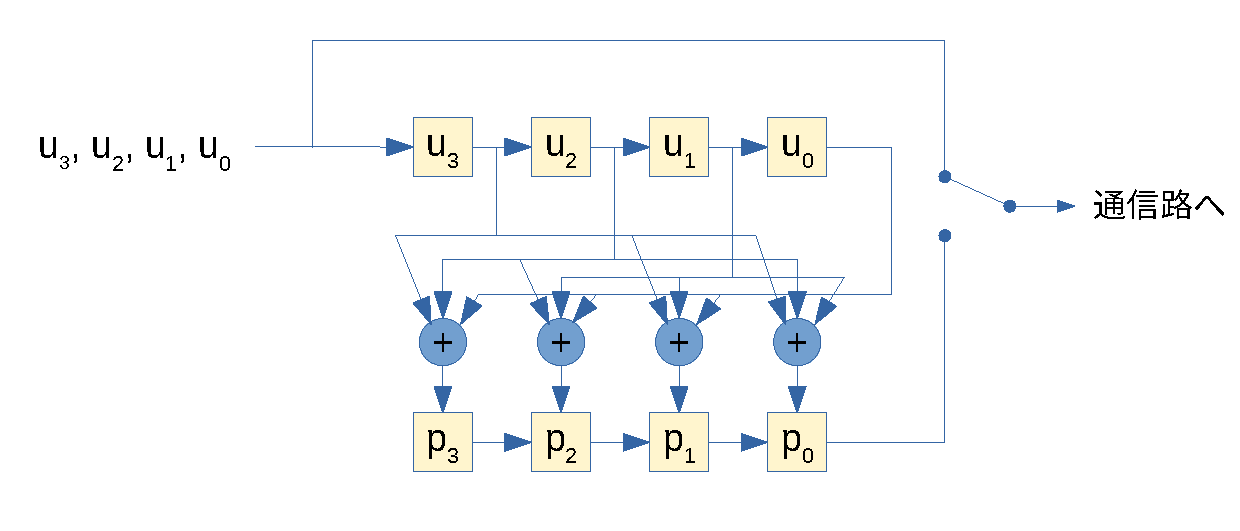
\includegraphics[scale=0.7]{figures/circuit001.pdf}
  \end{center}
  \caption{符号化回路
  \label{fig:encoding-circuit}
  }
\end{figure}

\subsection{シンドローム計算回路}
図\ref{fig:calc-syndrome}に示す。

\begin{figure}[htbp]
  \begin{center}
  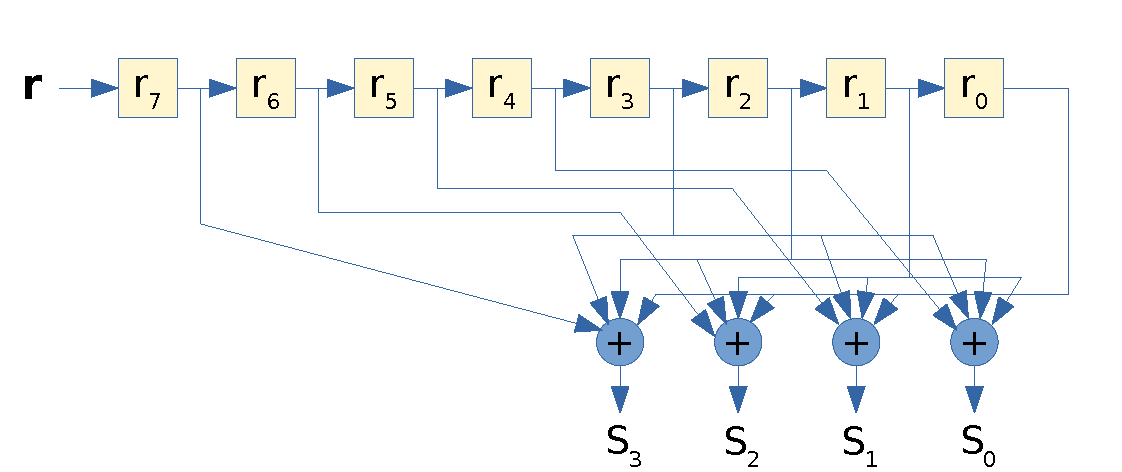
\includegraphics[scale=0.7]{figures/calc_syndrome001.pdf}
  \end{center}
  \caption{シンドローム計算回路
  \label{fig:calc-syndrome}
  }
\end{figure}

\subsection{重み分布と誤りを検出できない確率}
表\ref{table:all-code}より、重み分布は表\ref{table:weight-dist}となる。

\begin{table}[hbtp]
  \caption{重み分布}
  \label{table:weight-dist}
  \centering
  \begin{tabular}{|c|ccc|}
    \hline
    $i$ & 0 & 4 & 8 \\ \hline
    $A_i$ & 1 & 14 & 1 \\ \hline
  \end{tabular}
\end{table}

$p=0.01$のとき、誤りを検出できない確率は
\begin{eqnarray*}
  P_U(E) &=& \Sigma_{i=1}^{n}{A_ip^i(1-p)^{n-i}} \\
  &=& 14p^4(1-p)^4+1p^8(1-p)^0 \\
  &\simeq& 1.345 \times 10^{-7}
\end{eqnarray*}

\subsection{双対符号}
\eqref{eq:parity-check-matrix}の検査行列${\bm H}$を組織符号に変換すると、
\begin{equation*}
  \begin{bmatrix}
    0 & 1 & 1 & 1 \\
    1 & 1 & 1 & 0 \\
    1 & 1 & 0 & 1 \\
    1 & 0 & 1 & 1
  \end{bmatrix}
  \begin{bmatrix}
    0 & 1 & 1 & 1 & 1 & 0 & 0 & 0 \\
    1 & 1 & 1 & 0 & 0 & 1 & 0 & 0 \\
    1 & 1 & 0 & 1 & 0 & 0 & 1 & 0 \\
    1 & 0 & 1 & 1 & 0 & 0 & 0 & 1
  \end{bmatrix}=
  \begin{bmatrix}
    1 & 0 & 0 & 0 & 0 & 1 & 1 & 1 \\
    0 & 1 & 0 & 0 & 1 & 1 & 1 & 0 \\
    0 & 0 & 1 & 0 & 1 & 1 & 0 & 1 \\
    0 & 0 & 0 & 1 & 1 & 0 & 1 & 1
  \end{bmatrix}
\end{equation*}
より、生成行列${\bm G}$と等しくなる。

\section{(7,4)ハミング符号の復号誤り率の上限}
BSCにおける復号誤り率の上限は
\begin{equation*}
  P_{\rm max}(E) = \Sigma_{i=t+1}^{n}
  \begin{pmatrix}
    n \\ i
  \end{pmatrix}
  p^i(1-p)^{n-i}
\end{equation*}
なので、(7,4)ハミング符号の場合
\begin{equation*}
  P_{\rm max}(E) = \Sigma_{i=2}^{7}
  \begin{pmatrix}
    n \\ i
  \end{pmatrix}
  p^i(1-p)^{7-i}
\end{equation*}
である。二項定理より、
\begin{eqnarray*}
  1^n&=&((1-p)+p)^n=\Sigma_{i=0}^n
  \begin{pmatrix}
    n \\ i
  \end{pmatrix}
  p^i(1-p)^{n-i} \\
  &=&\Sigma_{i=0}^{t}
  \begin{pmatrix}
    n \\ i
  \end{pmatrix}
  p^i(1-p)^{n-i}+
  \Sigma_{i=t+1}^{n}
  \begin{pmatrix}
    n \\ i
  \end{pmatrix}
  p^i(1-p)^{n-i}
\end{eqnarray*}
となるので、
\begin{eqnarray*}
  P_{\rm max}(E)&=&\Sigma_{i=2}^{7}
  \begin{pmatrix}
    n \\ i
  \end{pmatrix}
  p^i(1-p)^{7-i}
  =1-\Sigma_{i=0}^{1}
  \begin{pmatrix}
    n \\ i
  \end{pmatrix}
  p^i(1-p)^{7-i} \\
  &=& 1-\left(
    1p^0(1-p)^{7}+7p^1(1-p)^{6}
  \right)=1-(1-p)^6(1-6p)
\end{eqnarray*}
と簡略化できる。これを$10^{-5} \leq p \leq 10^{-1}$の範囲で
プロットしたものが図\ref{fig:error-max}である。

\begin{figure}[htbp]
  \begin{center}
  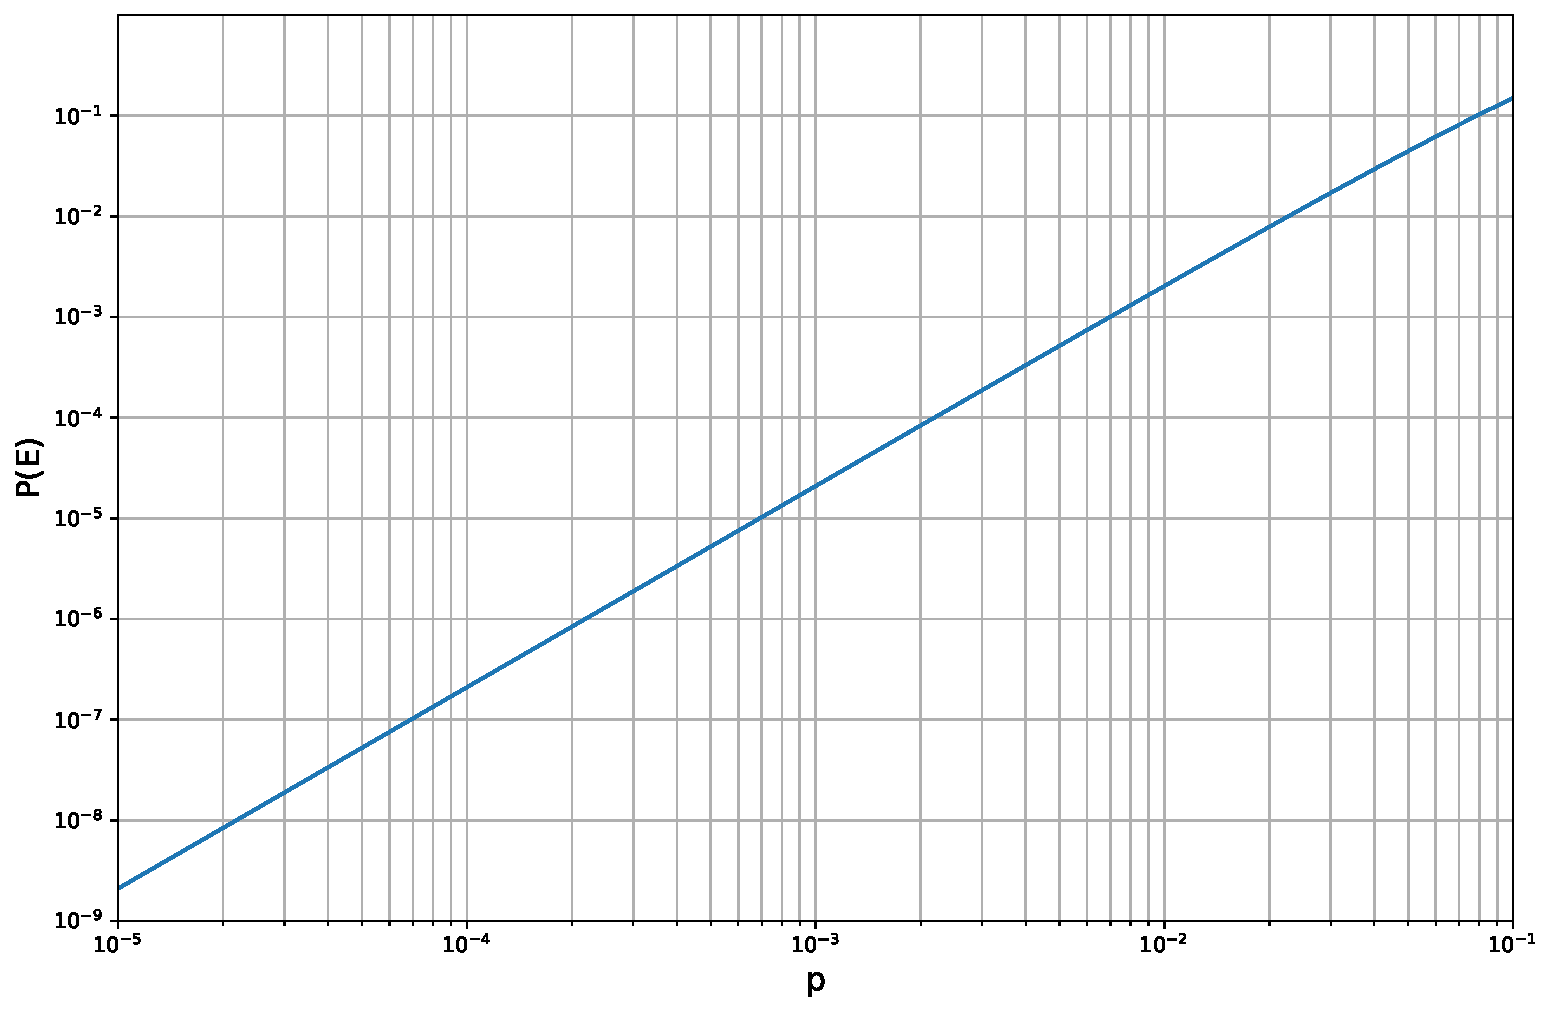
\includegraphics[scale=0.5]{figures/test.pdf}
  \end{center}
  \caption{(7,4)ハミング符号の復号誤り率の上限
  \label{fig:error-max}
  }
\end{figure}

\section{$d_{\rm min} \geq 2t+1$の(n,k)線形符号の場合}
符号長$n$の符号で、各誤りビット数の誤りパターン数を整理すると
表\ref{table:error-bits-num}になる。なお、
${}_nC_t$は$\binom{n}{t}$
と同じ意味なので$\binom{n}{t}$に統一する。
\begin{table}[hbtp]
  \caption{誤りビット数と誤りパターン数}
  \label{table:error-bits-num}
  \centering
  \begin{tabular}{|cc|}
    \hline
    誤りビット数 & 誤りパターン数 \\ \hline \hline
    0 & $\binom{n}{0}$ \\ \hline
    1 & $\binom{n}{1}$ \\ \hline 
    2 & $\binom{n}{2}$ \\ \hline 
    $\vdots$ & $\vdots$ \\ \hline
    $t$ & $\binom{n}{t}$ \\ \hline
    $\vdots$ & $\vdots$ \\ \hline
    $n$ & $\binom{n}{n}$ \\ \hline
  \end{tabular}
\end{table}
表\ref{table:error-bits-num}より、$t$ビット以下の誤りパターン数は
\[
  % \Sigma_{i=0}^{t}{\binom{n}{i}}
  \binom{n}{0}+\binom{n}{1}+\binom{n}{2}+\cdots \binom{n}{t}
\]
である。
$d_{\rm min} \geq 2t+1$の符号は$t$ビット以下の誤りを全て
訂正可能であり、(n,k)線形符号が訂正可能な誤りパターン数は
$2^{n-k}$なので、
\begin{eqnarray*}
  % 2^{n-k} \geq \Sigma_{i=0}^{t}{\binom{n}{i}}
  2^{n-k} \geq \binom{n}{0}+\binom{n}{1}+\binom{n}{2}+\cdots \binom{n}{t} \\
  \therefore n-k \geq \log_2\left(\binom{n}{0}+\binom{n}{1}+\binom{n}{2}+\cdots \binom{n}{t}\right)
\end{eqnarray*}


\end{document}